\chapter{Experiments and Evaluations}
\label{ch:experiments}

This chapter presents details of the experiments and evaluations for the proposed test scripts in the previous chapter.
First, we describe the environment setup for testing process.
Subsequently, we present all the experiments along with evaluation and assessment for each of them.

\section{Experimental environment}

\subsection{Hardware configurations}
All test suites are conducted with the hardware configurations as shown in table \ref{tab:hw}:

\begin{table}[H]
	\centering
	\caption{Hardware configuration for testing process}	
	\label{tab:hw}
	\begin{tabularx}{0.65\textwidth}{ll}
		\toprule
		Phone & ASUS Zenfone 5 \\
			  & Resolution 720 x 1280 pixels \\
			  & Screen 5'' 6.22 cm x 11.06 cm \\
			  & Android 5.0.1\\
		\midrule 
		Phone & Sony XPeria L \\
			  & Resolution 480 x 850 pixels \\
			  & Screen 4.3'' 5.40 cm x 9.60 cm \\
			  & Android 4.2.2\\
		\midrule 
		Robot & Self-construct Delta Robot \\
			  & \begin{minipage}{0.25\linewidth}
			\centering
			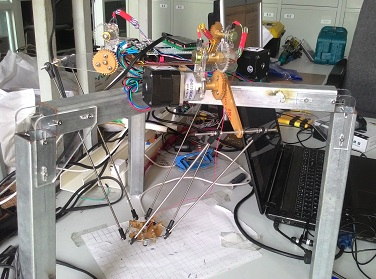
\includegraphics[width=0.8\linewidth]{Chapters/Fig/delta_robot.jpg}
		\end{minipage} \\
		\midrule 
		Computer & Windows PC \\
		\bottomrule
	\end{tabularx}
\end{table}

\subsection{Supporting software}
Beside running this application, we are required to have the following software installed on the computer.

	\begin{itemize}
		\item[--] \textbf{Android platform tool}: command line tools for communicate with Android device.
		\item[--] \textbf{Droid@Screen}: application letting us capture Android screen to PC.
	\end{itemize}

\section{Experiments and Evaluations}
This section gives the details of all experiments that we have conducted to verify and evaluate the accuracy of Delta robot as well as the whole Testing System proposed in the previous chapter.

\subsection{Experiment 1: Test robot accuracy}
\subsubsection{Experimental purpose}

\subsubsection{Experimental setup}

\subsubsection{Experimental results}
[Some pictures here]

\subsection{Experiment 2: Set alarm}
\subsubsection{Experimental purpose}

\subsubsection{Experimental setup}

\subsubsection{Experimental results}

\section{Analysis and evaluation}
\subsection{Results analysis}
\begin{table}[H]
	\centering
	\caption{Test results statistic}	
	\label{tab:result_stat}
	\begin{tabularx}{0.65\textwidth}{l|rrr}
		\hline
		Test case & Successful & Failed & Number of tests \\
		\hline
		Simple Click & 10 & 0 & 10 \\
		Set Alarm & 5 & 5 & 10 \\
		\hline
		Total & 15 & 15 & 20 \\
		\hline
		\textbf{Rate} & \textbf{0.50} & \textbf{0.50} & \textbf{1.00} \\
		\hline
	\end{tabularx}
\end{table}

\subsection{Conclusion:} //TODO: [edit this]With both VGGNet and AlexNet as the CNN module of the model, Adam gives the best results in terms of the model convergence rate. Hence, it will be used as the optimization method in the subsequent experiments.
